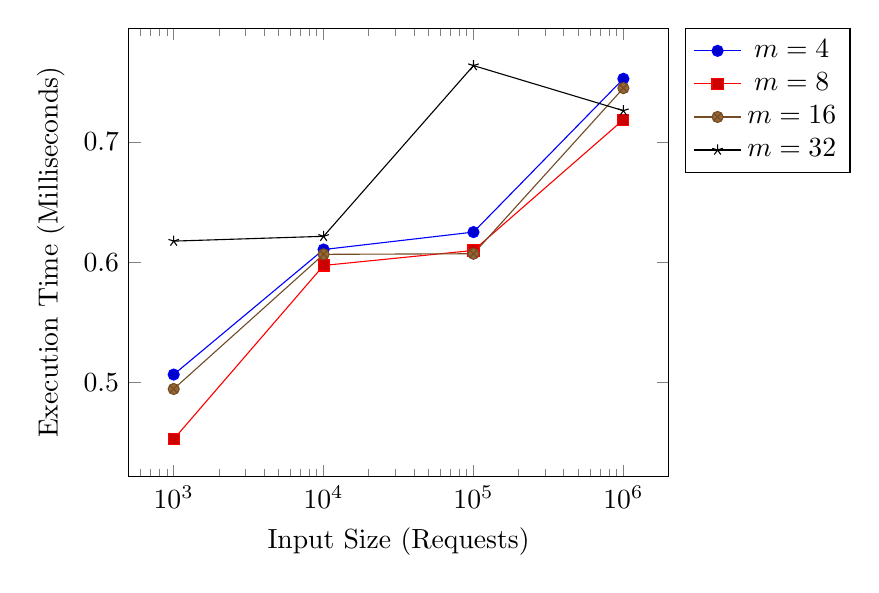
\begin{tikzpicture}
	\begin{axis}
		[
			xlabel={Input Size (Requests)},
			ylabel={Execution Time (Milliseconds)},
			legend pos=outer north east,
			domain=1:1000000,
			xmode=log,
		]
		\addplot+[cycle list name=color list]
			coordinates {
				(1000, 0.5065)
				(10000, 0.6105)
				(100000, 0.625)
				(1000000, 0.7525)
			};
		\addlegendentry{$m=4$}
		\addplot+[cycle list name=color list]
			coordinates {
				(1000, 0.45275)
				(10000, 0.59725)
				(100000, 0.60975)
				(1000000, 0.7185)
			};
		\addlegendentry{$m=8$}
		\addplot+[cycle list name=color list]
			coordinates {
				(1000, 0.4945)
				(10000, 0.6065)
				(100000, 0.607)
				(1000000, 0.74475)
			};
		\addlegendentry{$m=16$}
		\addplot+[cycle list name=color list]
			coordinates {
				(1000, 0.6175)
				(10000, 0.6215)
				(100000, 0.7635)
				(1000000, 0.726)
			};
		\addlegendentry{$m=32$}
	\end{axis}
\end{tikzpicture}
